% $Id: CONTENT.tex 12318 2010-09-24 12:03:43Z alexandra $
% Local Variables:
% ispell-check-comments: nil
% Local IspellDict: american
% End:
% --------------------------------------------------------
% User documentation
% copyright by BREDEX GmbH 2004
% --------------------------------------------------------

\app{} uses a graphical installer to make installation as straightforward as possible. 

You don't need administrative privileges to install \app{}, but the folder where the software will be installed must be writable and allow program execution.

See the following sections for information on installing \app{} on Windows and Unix systems. For installation on  other platforms, please follow the Unix installation procedure, and adapt the instructions as necessary.

\section{Installation procedure}
 
The installation process for \app{} consists of the following parts:

\begin{enumerate}
\item Install the software on your computer.
\item Use the configuration tool \bxpref{custInst} to define if logs should be kept, and where the license file should be stored. Using the configuration tool is optional; if you don't use it, defaults will be used.
\item Use the database tool to define what database to use. Using the database tool is optional; if you don't use it, defaults will be used.
\item Request a license and upload it to the license server via the license administrator \bxpref{license}. 
%\bxtipp{The license server cannot currently run on MAC OSX. Please install the license server on a separate system to use \app{} on MAC OSX. }
\end{enumerate}

\bxwarn{Please read the following paragraph for information on a known issue with an environment variable}

\begin{itemize}
\item There is a known problem with an environment variable which is installed with certain products, including other test tools, and may not be uninstalled when these products are uninstalled. 

\item The variable is called ''\_JAVA\_OPTION'' and causes problems for \app{} and possibly also for other Java-based software.

\item To see if this variable is installed on your computer, right-click on the ''my computer'' icon on your desktop and select ''properties''. 
\item In the dialog which appears, select the ''advanced'' tab and, at the bottom, click on the ''environment variables'' button. 
\item You will see a list of environment variables on the computer. 
\item If the ''\_JAVA\_OPTION'' variable is present, and you have uninstalled the program which used it, then you can simply remove the variable.
\end{itemize}

\section{\app{} components}

\app{} consists of a set of programs which are shown in the following figure(\bxfigref{gdcomponents}).

\begin{figure}
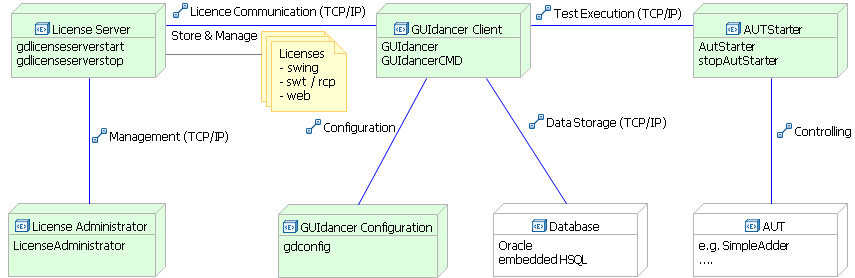
\includegraphics[width=16cm]{Installation/PS/standardInstallationDeployment}
\caption{\app{} components}
\label{gdcomponents}
\end{figure}

\begin{description}
\item [The \app{} client: ]{This is where test are created. Tests can also be executed from the client. You can think of this as the main application. The client can also run headless -- the command line client.}
\item [The \app{} configuration tool: ]{This tool configures the \app{} client. It specifies which \gddb{} to use, whether logging is activated and which license server to use to acquire licenses from.}
\item [The license server: ]{This application stores and manages all available licenses and distributes them to the \app{} clients which are configured to use this license server. Therefore, each client needs a TCP/IP connection to the computer on which the license server is running.}
\bxwarn{For MAC systems, the license server requires the development kit for the environment to run.}
\item [The license admnistrator: ]{This is the component that manages the license server(s). New licenses can be uploaded to the license server using the license administrator and invalid licenses removed. The license administrator also provides you with the serverID for the license server(s). The serverID is needed to request licenses in the \app{} shop.}
\item [The \gdagent{}:]{ This component is responsible for controlling the \gdaut{} during test execution. It must be installed on the machine(s) where you want your \gdaut{} and tests to run. The \gdagent{} itself requires no license. It does however require a network connection to communicate with the \app{} client. }
\end{description}

During the installation process you can choose between different bundles of these programs to be installed (\bxfigref{figComponents}):

\begin{itemize}
\item \app{}, this bundle includes
	\begin{itemize}
	\item the \app{} Client,
	\item the \app{} configuration tool and database tool,
	\item and the License Administrator.
	\end{itemize}
\item \gdagent{}, this bundle includes only the \gdagent{}, which handles the testing
of your \gdaut{}.
\item \app{} Documentation, this bundle includes the PDF Documentation.
\item License Server, this bundle includes the 
	\begin{itemize}
	\item License Server,
	\item and the License Administrator.
	\end{itemize}
\end{itemize}


 
